\section{Task 3: Multimodal Clustering of Material Types}
\label{sec:t3}
% Numbers: kode/results/task3/results.json (python run_all.py --task 3). Supporting figures: Appendix A.2.

We group 36{,}000 unlabeled laboratory material samples into material types from paired
$64 \times 64$ microstructure images and 128-bin composition spectra, recorded across two
microscopes (M1: 21{,}636 samples, 60.1\%; M2: 14{,}364 samples, 39.9\%). Using SimCLR
self-supervised encoders~\cite{chen2020simclr} fused via L2-normalized concatenation and
agglomerative clustering, we identify \textbf{7 well-separated material clusters} with near-perfect
neighborhood purity (99.5--100.0\%) and zero microscope leakage (Cram\'er's $V = 0.0096$).
Supporting figures are in Appendix~\ref{app:t3}.

\subsection{Exploration of image and spectrum distortions}
\label{sec:t3-eda}

\paragraph{Image distortions.} Comparing microscopes reveals a strong systematic shift
(Fig.~\ref{fig:t3-eda-mic}): M2 images are substantially brighter than M1 (mean intensity 146.1 vs.\
127.8) and carry higher high-frequency texture/noise energy (high-frequency share 8.69\% vs.\
5.13\%), while within-image contrast is almost identical (std 19.9 vs.\ 19.7). In addition, 34.9\%
of images exhibit directional microstructure with nearly uniform orientation distribution (max/min
histogram ratio 1.40), confirming arbitrary sample rotation and scale variations.

\paragraph{Spectrum distortions.} Composition spectra suffer from four nuisances
(Fig.~\ref{fig:t3-eda-spec}): narrow spikes affect 22.2\% of samples (mean 0.253 spikes/sample,
median amplitude 2.46 vs.\ noise $\sigma = 0.042$), baseline offset (edge SD 0.336), linear tilt
(tilt SD 0.399), and horizontal wavelength shifts (mean $|\text{shift}| = 1.86$ bins, 95th
percentile 4.0 bins).

\subsection{Unsupervised representation learning}
\label{sec:t3-ssl}

\paragraph{Preprocessing and distortion-targeted augmentations.} Images are standardized per sample
(removing global brightness and contrast differences between M1 and M2). Spectra are cleaned before
encoding with a 5-bin median filter to remove spikes, followed by subtracting a 61-bin rolling
median to remove baseline offset/tilt, and L2-normalizing each spectrum. To make embeddings
invariant to the remaining nuisances, we train separate SimCLR~\cite{chen2020simclr} encoders
(NT-Xent temperature $T=0.2$, batch size 512, seed 0, mixed precision on a Colab T4 GPU; Python
3.13, PyTorch 2.14, NumPy 2.4.6, scikit-learn 1.6.1, umap-learn 0.5.12):
\begin{itemize}
  \item \textbf{Image encoder (2D ResNet, 256-d $\to$ PCA 32-d):} four residual stages (32, 64, 128,
  256 channels), trained 60 epochs (final NT-Xent loss 2.78) with full $360^\circ$ rotation, random
  horizontal flip, scale $[0.8, 1.25]$, translation $\pm 10\%$, gamma jitter, and Gaussian blur
  (targeting M1/M2 sharpness and arbitrary orientation/scale).
  \item \textbf{Spectrum encoder (1D CNN, 256-d $\to$ PCA 32-d):} six strided 1D conv blocks
  (width 7), trained 100 epochs (final loss 2.38) with random horizontal shift up to $\pm 4$ bins,
  mild amplitude scaling, and additive noise (targeting calibration shift and residual noise).
\end{itemize}

\subsection{Two modalities and fusion}
\label{sec:t3-fusion}

We compare four 32-d/64-d embeddings: \texttt{img} only, \texttt{spec} only, \texttt{joint}
(a 20-epoch feature-level MLP fusion head trained jointly with contrastive + cross-modal CLIP
loss), and \texttt{concat} (64-d concatenation of the L2-normalized 32-d \texttt{img} and
\texttt{spec} embeddings). Table~\ref{tab:t3-fusion} shows that \texttt{joint} collapses toward the
spectrum modality (kNN overlap 0.470 with \texttt{spec} vs.\ 0.005 with \texttt{img}; silhouette
0.254), whereas \texttt{concat} achieves higher silhouette (0.320) and balanced kNN overlap with
both modalities (0.105 image, 0.094 spectrum). We therefore select \texttt{concat}.

\begin{table}[t]
  \centering
  \caption{Comparison of single-modality and fused representations on all 36{,}000 samples (from
  \texttt{kode/results/task3/results.json}). Microscope leak is linear probe accuracy for M1 vs.\ M2
  (majority baseline 60.1\%).}
  \label{tab:t3-fusion}
  \small
  \begin{tabular}{lrrrrrrr}
    \toprule
    Embedding & Dim & Best $K$ (sil.) & Silhouette & DB & Mic.\ leak & kNN ov.\ img & kNN ov.\ spec \\
    \midrule
    \texttt{img}    & 32 & 6  & 0.318 & 1.252 & 69.4\% & 1.000 & 0.002 \\
    \texttt{spec}   & 32 & 4  & 0.324 & 1.371 & 60.0\% & 0.002 & 1.000 \\
    \texttt{joint}  & 32 & 15 & 0.254 & 1.482 & 59.9\% & 0.005 & 0.470 \\
    \textbf{\texttt{concat}} & 64 & 5 & \textbf{0.320} & \textbf{1.275} & 70.2\% & \textbf{0.105} & \textbf{0.094} \\
    \bottomrule
  \end{tabular}
\end{table}

\paragraph{What is lost with one modality.} Figure~\ref{fig:t3-umap} (middle and right) and the
pairwise separability matrices (Fig.~\ref{fig:t3-pairs}) demonstrate directly why neither modality
suffices alone:
\begin{itemize}
  \item \textbf{Image-only loses Clusters 1 vs.\ 5:} their microstructures are indistinguishable
  ($d'_{\text{img}} = 0.06$), so image-only embeddings merge them into a single blob; they separate
  cleanly in composition spectra ($d'_{\text{spec}} = 6.77$).
  \item \textbf{Spectrum-only loses Clusters 3 vs.\ 4 (and merges 2 vs.\ 6):} Clusters 3 and 4 have
  virtually identical spectra ($d'_{\text{spec}} = 0.06$) and separate only in microstructure images
  ($d'_{\text{img}} = 6.64$).
\end{itemize}

\begin{figure}[t]
  \centering
  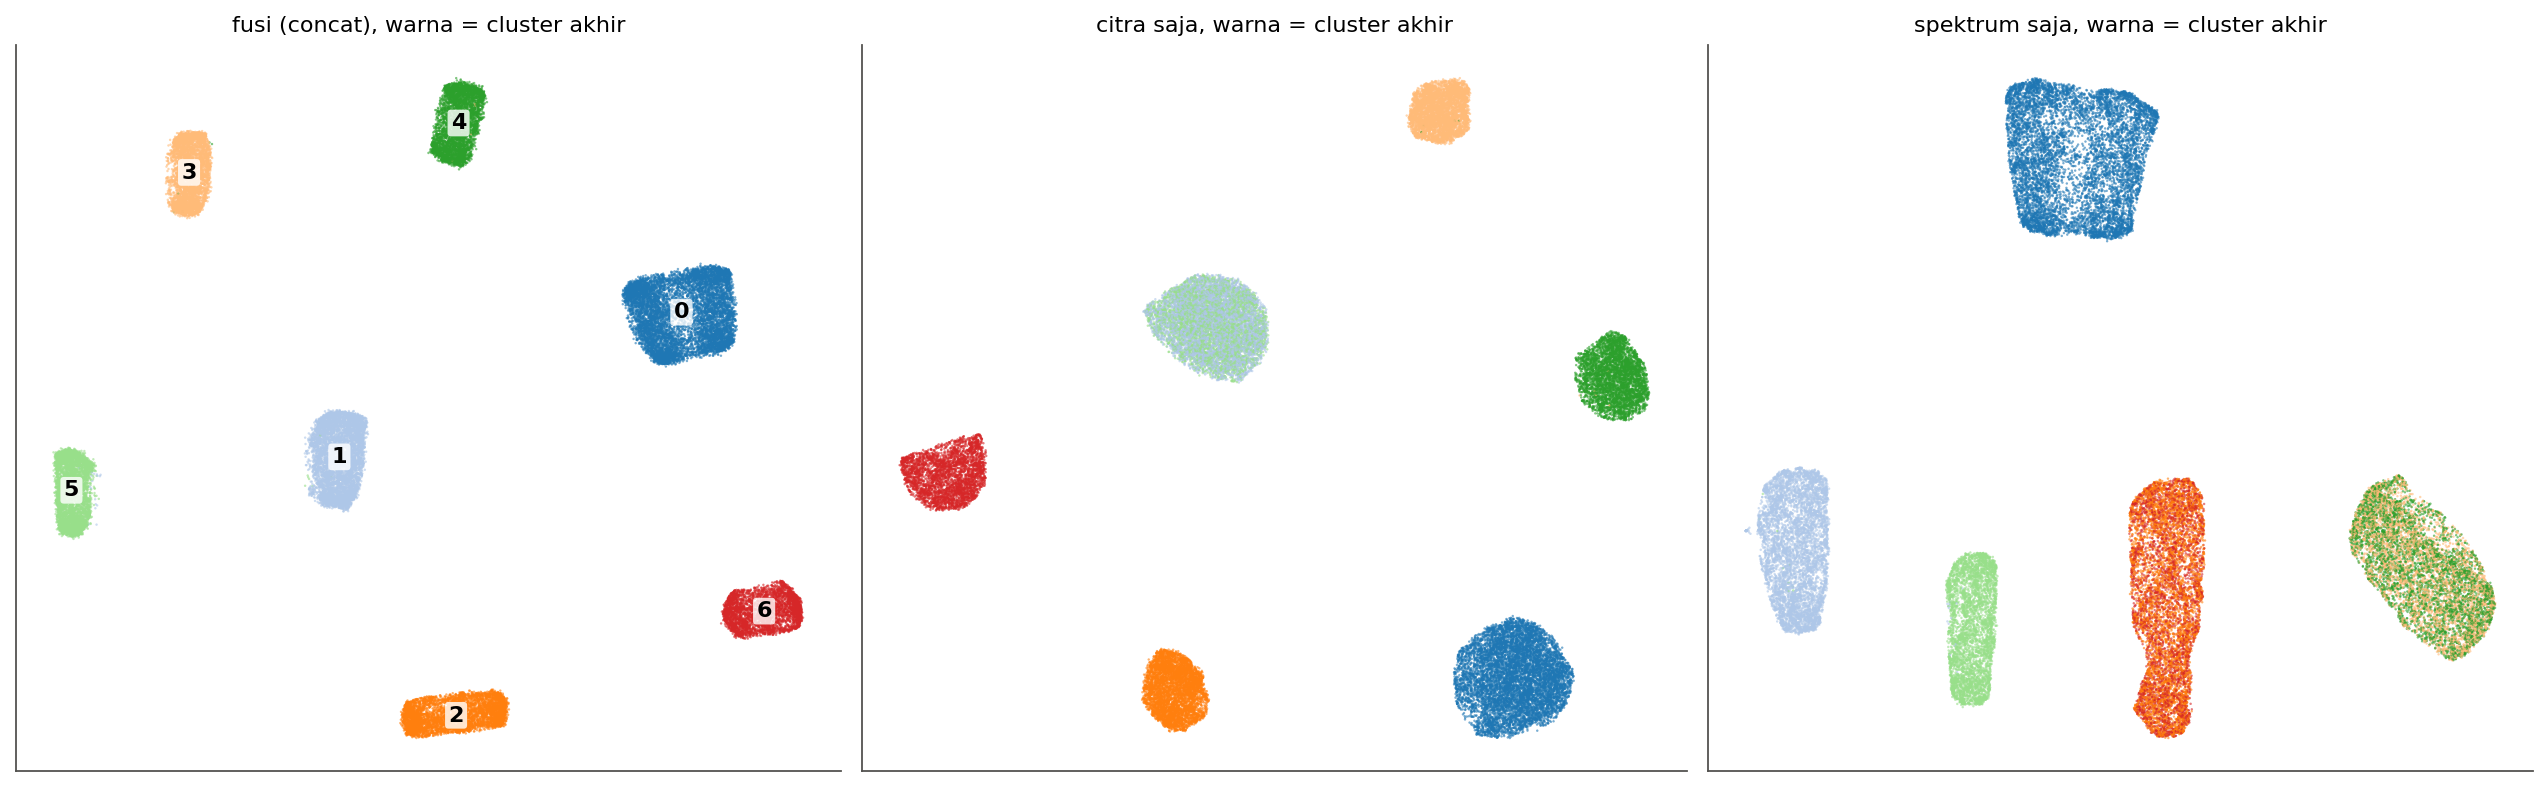
\includegraphics[width=\linewidth]{t3_umap_clusters}
  \caption{UMAP projections~\cite{mcinnes2018umap} coloured by final cluster ID (0--6). Left: fused
  \texttt{concat} embedding cleanly separates all 7 islands. Middle: image-only merges clusters 1
  and 5. Right: spectrum-only merges clusters 3 and 4 (as well as 2 and 6).}
  \label{fig:t3-umap}
\end{figure}

\subsection{Number of clusters and clustering methods}
\label{sec:t3-cluster}

\paragraph{Choosing $K = 7$ over $K = 5$.} We scanned $K = 2 \dots 16$ across six criteria
(Fig.~\ref{fig:t3-k}): five criteria (silhouette 0.320, Davies--Bouldin 1.275,
Calinski--Harabasz 9{,}463, bootstrap ARI stability 0.957, and cross-modal ARI 0.914) peak at
$K = 5$, while GMM BIC decreases monotonically to $K = 16$. Checking the kNN graph ($k = 15$ and
$k = 30$) explains why: the graph has \textbf{5 connected components} (sizes 10{,}043, 8{,}685,
8{,}637, 4{,}979, 3{,}656), giving four zero Laplacian eigenvalues, \emph{followed by two more
near-zero eigenvalues} ($0.0016$ and $0.0031$ at $k=15$) before a $10\times$ spectral gap to the
seventh ($0.0311$). Those two near-zero eigenvalues correspond to two components that each split
into two single-modality islands ($10{,}043 = 5{,}790 + 4{,}253$ for Clusters 1 vs.\ 5;
$8{,}637 = 4{,}341 + 4{,}296$ for Clusters 3 vs.\ 4) with a graph cut of only 0.1--0.2\%. Because
single-modality differences are real distinct material types, we override $K_{\text{auto}} = 5$ to
\textbf{$K = 7$} (based strictly on internal graph and pairwise evidence, never the hidden
reference).

\begin{figure}[t]
  \centering
  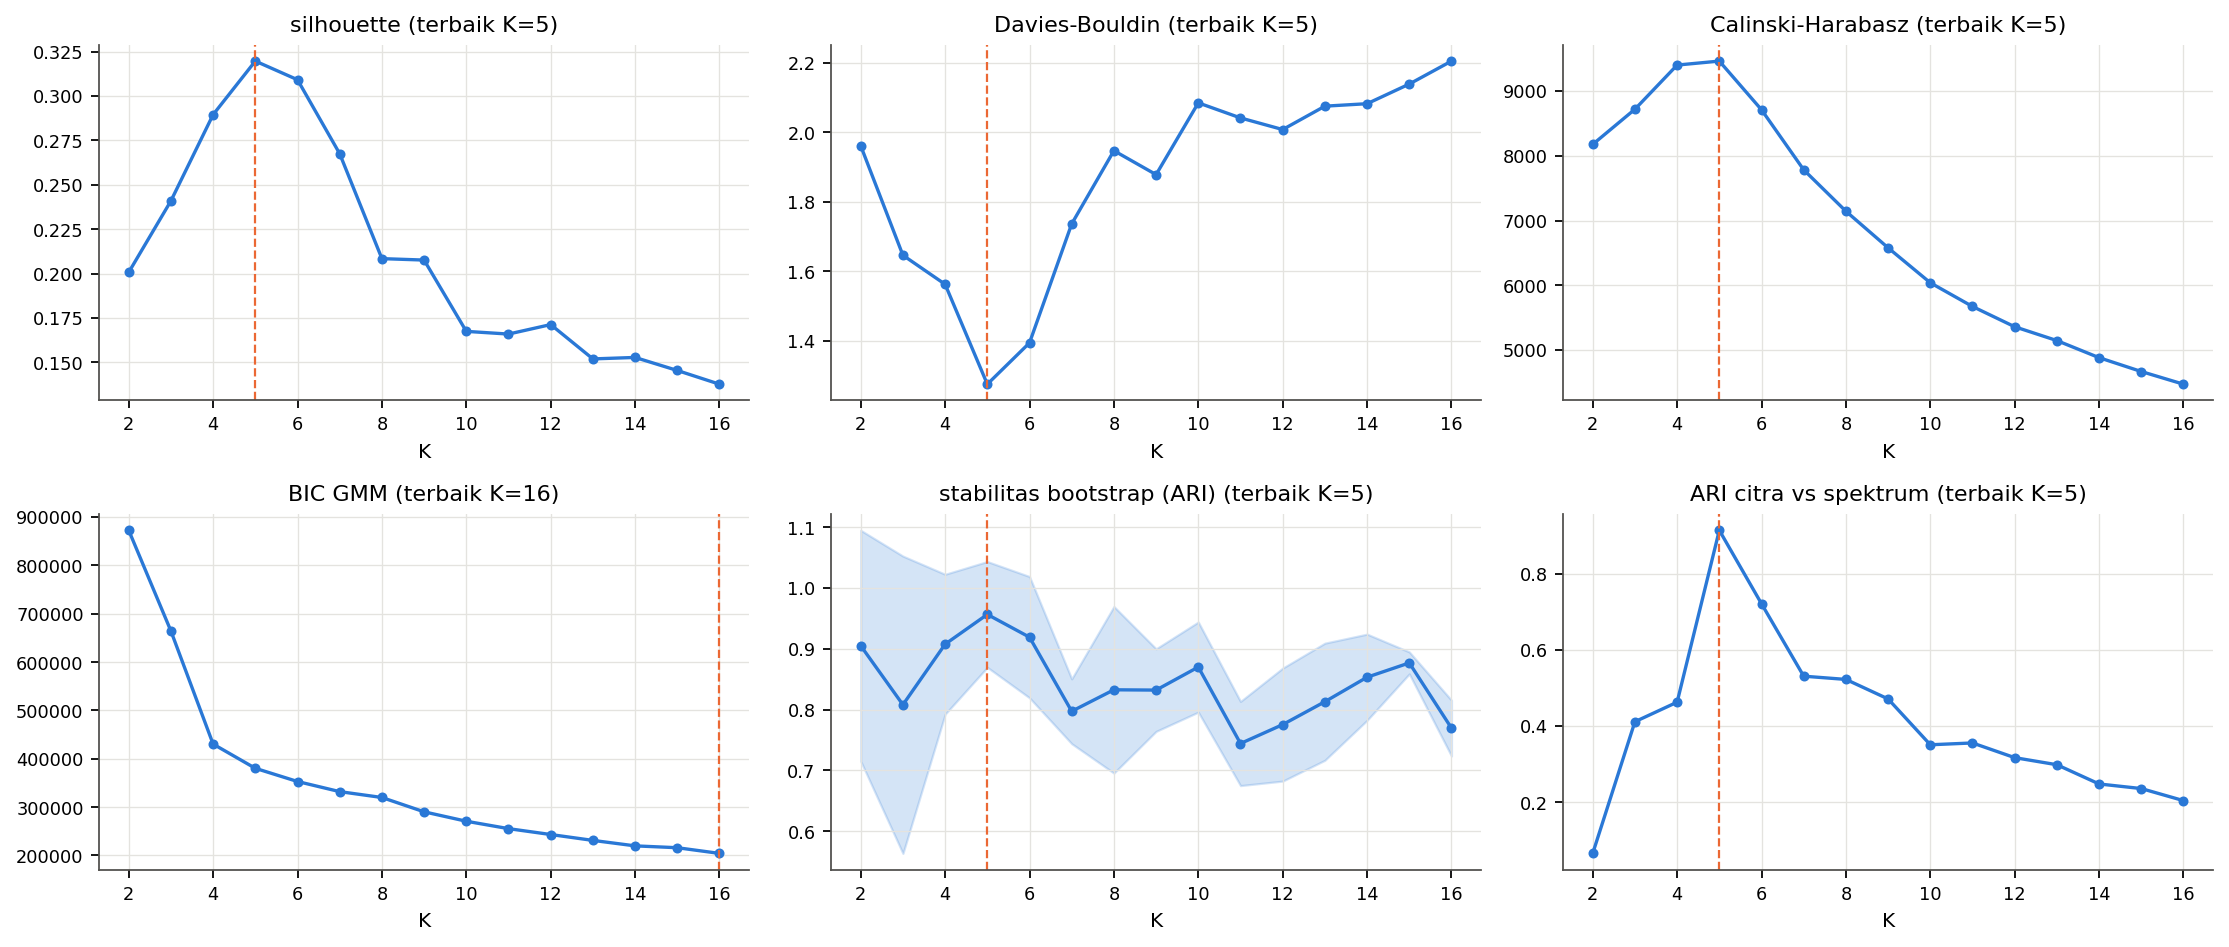
\includegraphics[width=\linewidth]{t3_k_criteria}
  \caption{Cluster-count scan ($K=2 \dots 16$) across six internal criteria on the fused
  \texttt{concat} embedding. Five criteria vote for $K=5$ (the 5 connected components of the kNN
  graph), while Laplacian spectral gap and single-modality island analysis motivate $K=7$.}
  \label{fig:t3-k}
\end{figure}

\paragraph{Comparing five clustering methods (including DEC).} At $K = 7$, we compare KMeans,
full-covariance GMM, Ward/average Agglomerative clustering, kNN graph partitioning, and Deep
Embedded Clustering (DEC~\cite{xie2016dec}, a 60-epoch autoencoder refined for 60 KL-divergence
iterations). Table~\ref{tab:t3-methods} shows that KMeans (kNN cut 1.65\%) and DEC (silhouette
0.220, DB 1.994, kNN cut 2.24\%) cut across dense islands instead of following the thin bridges
between single-modality pairs. In contrast, \textbf{Agglomerative} (kNN cut 0.19\%), GMM (0.12\%),
and Graph partitioning (0.12\%) all recover the exact 7 islands cleanly. We select
\textbf{Agglomerative} on \texttt{concat} for \texttt{cluster.csv} (cluster sizes 3{,}656 to
8{,}685).

\begin{table}[t]
  \centering
  \caption{Clustering methods compared at $K = 7$ on the 64-d fused \texttt{concat} embedding.
  \texttt{kNN cut} is the share of kNN edges crossing between clusters (lower = respects dense
  islands).}
  \label{tab:t3-methods}
  \small
  \begin{tabular}{lrrrrrr}
    \toprule
    Method & Sil.\ fused & Sil.\ img & Sil.\ spec & DB & kNN cut & Seed ARI \\
    \midrule
    KMeans                 & 0.268 & 0.245 & 0.156 & 1.736 & 0.0165 & 0.930 \\
    GMM                    & 0.246 & 0.228 & 0.125 & 1.725 & 0.0012 & 0.784 \\
    \textbf{Agglomerative} & 0.246 & 0.228 & 0.125 & 1.728 & \textbf{0.0019} & --    \\
    Graph (kNN)            & 0.246 & 0.228 & 0.125 & 1.725 & 0.0012 & --    \\
    DEC~\cite{xie2016dec}  & 0.220 & 0.159 & 0.188 & 1.994 & 0.0224 & 0.723 \\
    \bottomrule
  \end{tabular}
\end{table}

\subsection{Visualization, hard-to-separate clusters, and microscope invariance}
\label{sec:t3-analysis}

Both UMAP (Fig.~\ref{fig:t3-umap}) and t-SNE~\cite{vandermaaten2008tsne} (Appendix
Fig.~\ref{fig:t3-tsne}) show seven compact islands with 99.5--100.0\% same-cluster kNN purity per
cluster. Coloring the UMAP by microscope and raw image brightness (Fig.~\ref{fig:t3-mic}) confirms
uniform mixing inside every cluster: M2 share sits within 39.2--40.7\% across all seven clusters
(dataset average 39.9\%; Cram\'er's $V = 0.0096$), verifying that clusters reflect material types
rather than microscope artifacts.

As shown in Fig.~\ref{fig:t3-pairs}, the only cluster pairs with any nonzero neighborhood overlap
are the two single-modality pairs: \textbf{Clusters 1 vs.\ 5} (overlap 0.45\%, $d'_{\text{img}} =
0.06$, $d'_{\text{spec}} = 6.77$) and \textbf{Clusters 3 vs.\ 4} (overlap 0.25\%, $d'_{\text{img}}
= 6.64$, $d'_{\text{spec}} = 0.06$). Every other pair has 0.00\% overlap ($d' \ge 8.8$ in at least
one modality). This explains why those two pairs have lower per-cluster silhouettes (0.116--0.158
for 1/5 and 0.224--0.232 for 3/4, versus 0.301--0.352 for 0/2/6): they share half of their
64-dimensional representation. Note transparently that overriding $K_{\text{auto}}=5 \to 7$ and
choosing Agglomerative by low \texttt{kNN cut} were guided by inspecting the internal graph and
pairwise structure after training.

\begin{figure}[t]
  \centering
  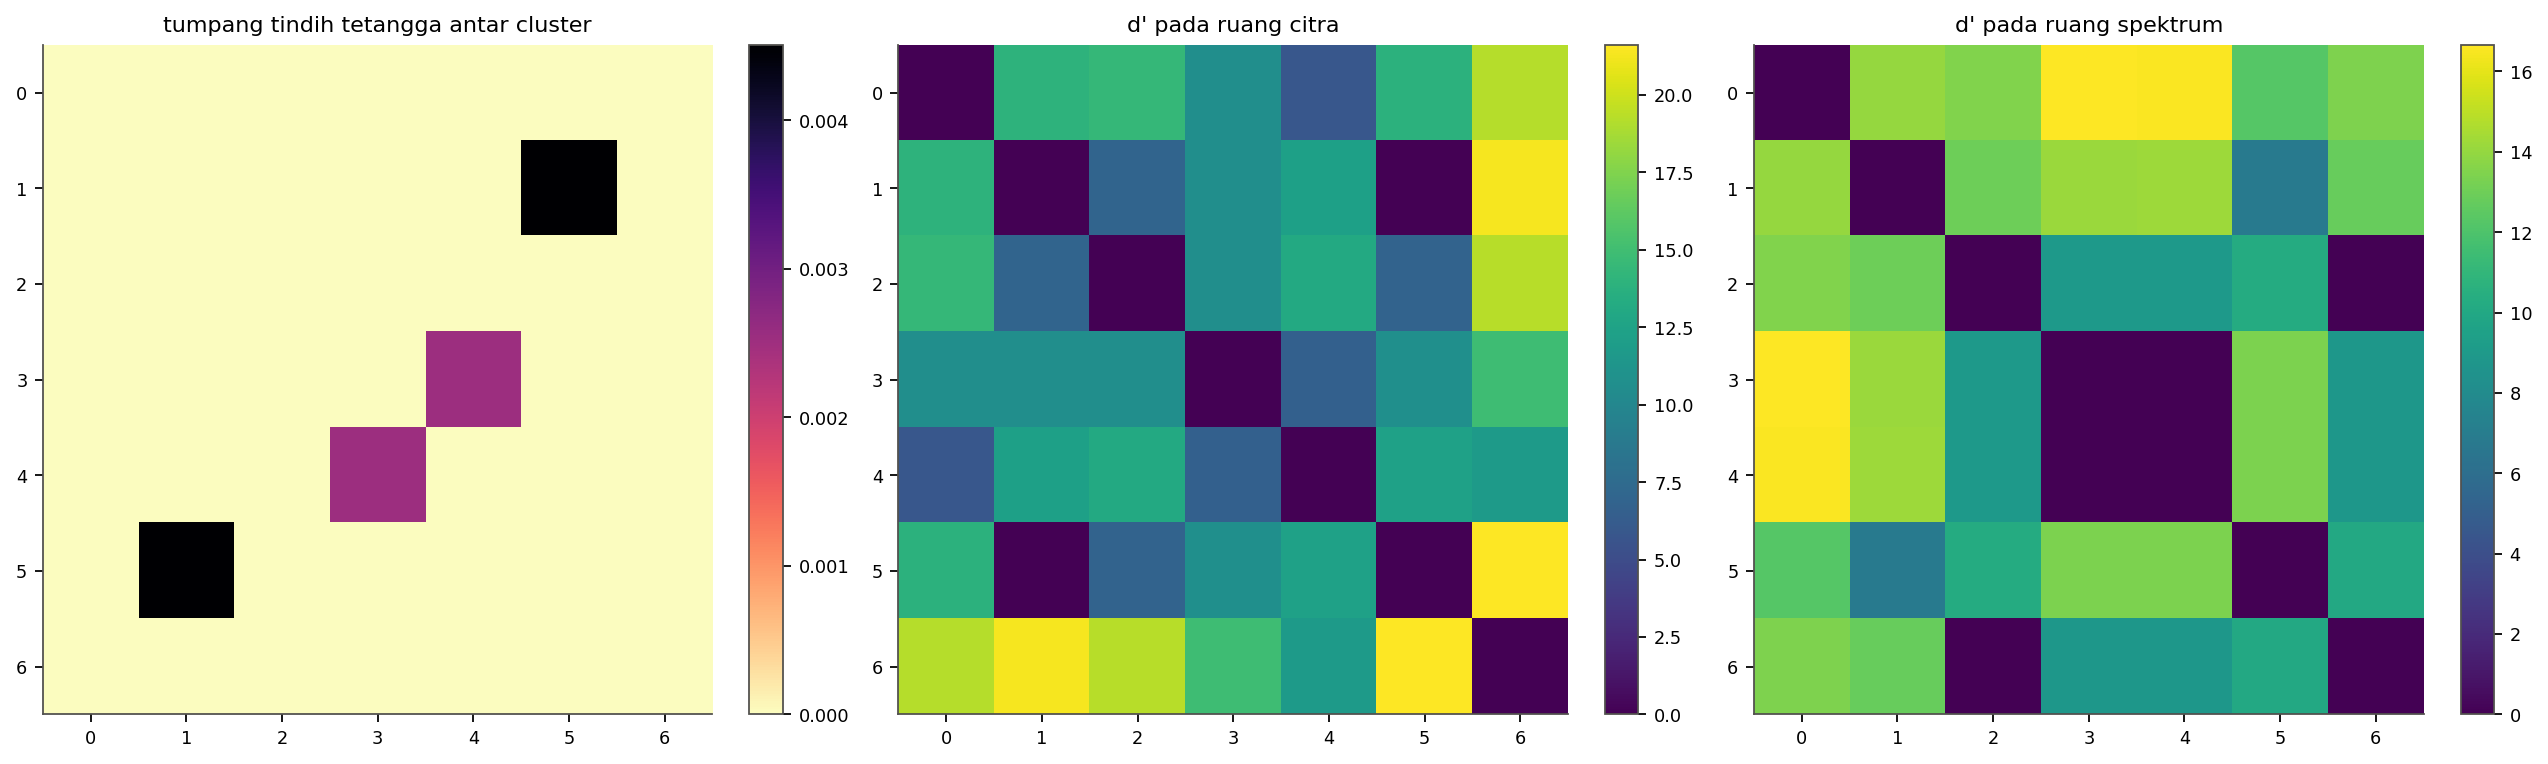
\includegraphics[width=\linewidth]{t3_pair_matrices}
  \caption{Pairwise cluster diagnostics at $K = 7$. Left: kNN boundary overlap (only pairs 1--5
  and 3--4 are nonzero, $\le 0.45\%$). Middle and right: $d'$ separation in image space vs.\
  spectrum space, confirming why single-modality clustering misses one of the two pairs.}
  \label{fig:t3-pairs}
\end{figure}

\begin{figure}[t]
  \centering
  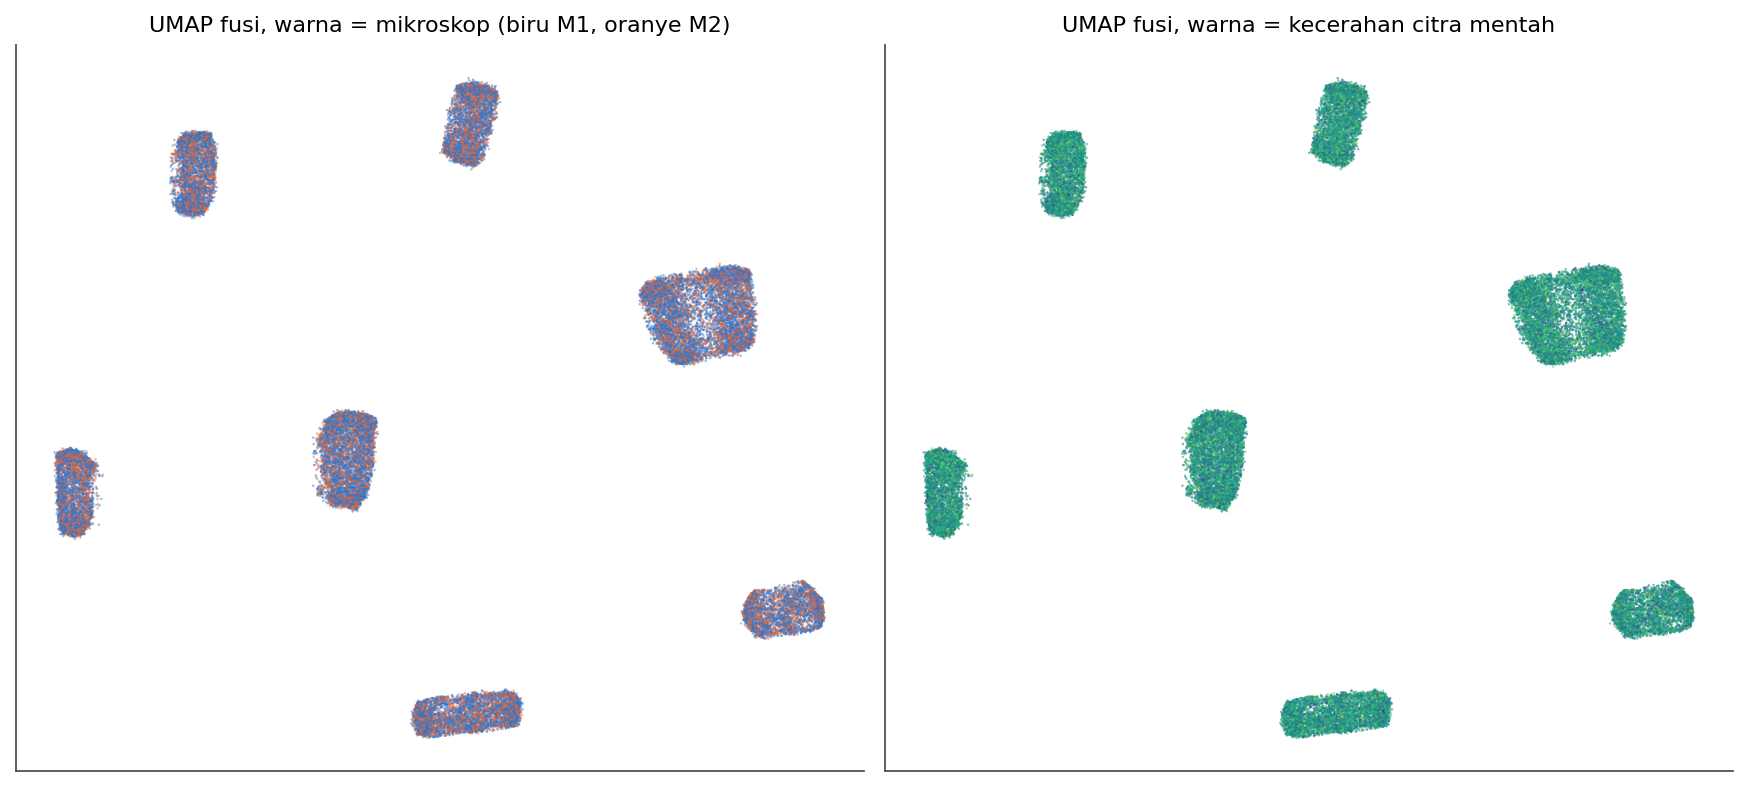
\includegraphics[width=\linewidth]{t3_umap_microscope}
  \caption{Microscope and brightness invariance check on the fused UMAP. Left: M1 (blue) and M2
  (orange) mix uniformly inside every island (Cram\'er's $V = 0.0096$). Right: raw image brightness
  shows no cluster-level bias.}
  \label{fig:t3-mic}
\end{figure}
